%=========================================================================
% sec-profile
%=========================================================================

\section{Profiling the Floyd-Warshall Algorithm}
\label{sec-profile}

\subsection{Identifying Bottlenecks}
\label{sec-profile-bottlenecks}

From the VTune profiling reports (Figure~\ref{fig-profile-bottlenecks-0}
and Figure~\ref{fig-profile-bottlenecks-1}), we can see that a large
proportion of the CPU time is spent in the function square, specifically
in lines 52, 54 and 51. Upon further inspection of the code, we observe
that in the innermost for-loop (line 52), we are accessing the array l at
strides of size n to iterate over elements in row i. Since the matrix is
stored in column-major order, accessing elements in a single row causes a
stride of size n, resulting in poor spatial locality and inefficient use
of the cache, thus contributing to the high CPU timing for that
particular line as reported in Figure~\ref{fig-profile-bottlenecks-1}.

\begin{figure}[h]
  \centering
  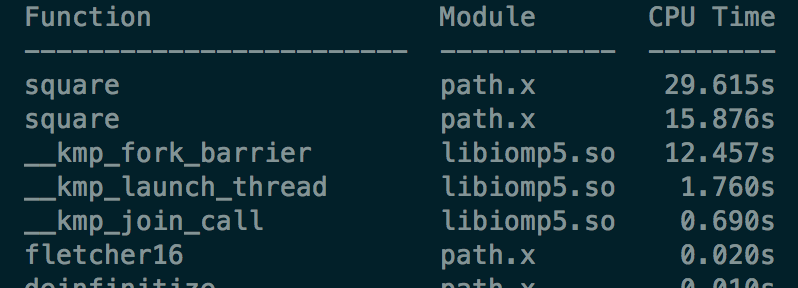
\includegraphics[width=0.7\tw]{fig-profile-bottlenecks-0.png}
  \caption{\textbf{VTune profiling output: Hotspots report (for n = 2000,
      p = 0.05)}}
  \label{fig-profile-bottlenecks-0}
\end{figure}

\begin{figure}[h]
  \centering
  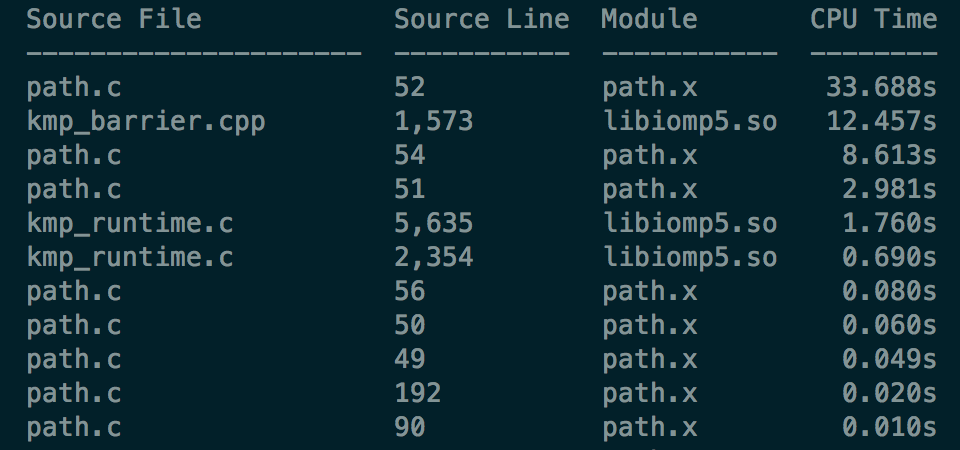
\includegraphics[width=0.7\tw]{fig-profile-bottlenecks-1.png}
  \caption{\textbf{VTune profiling output: (by line in source)}}
  \label{fig-profile-bottlenecks-1}
\end{figure}

\begin{center}
  \texttt{amplxe-cl -report hotspots -r r002hs -group-by source-line}
\end{center}

\begin{figure}[h]
  \centering
  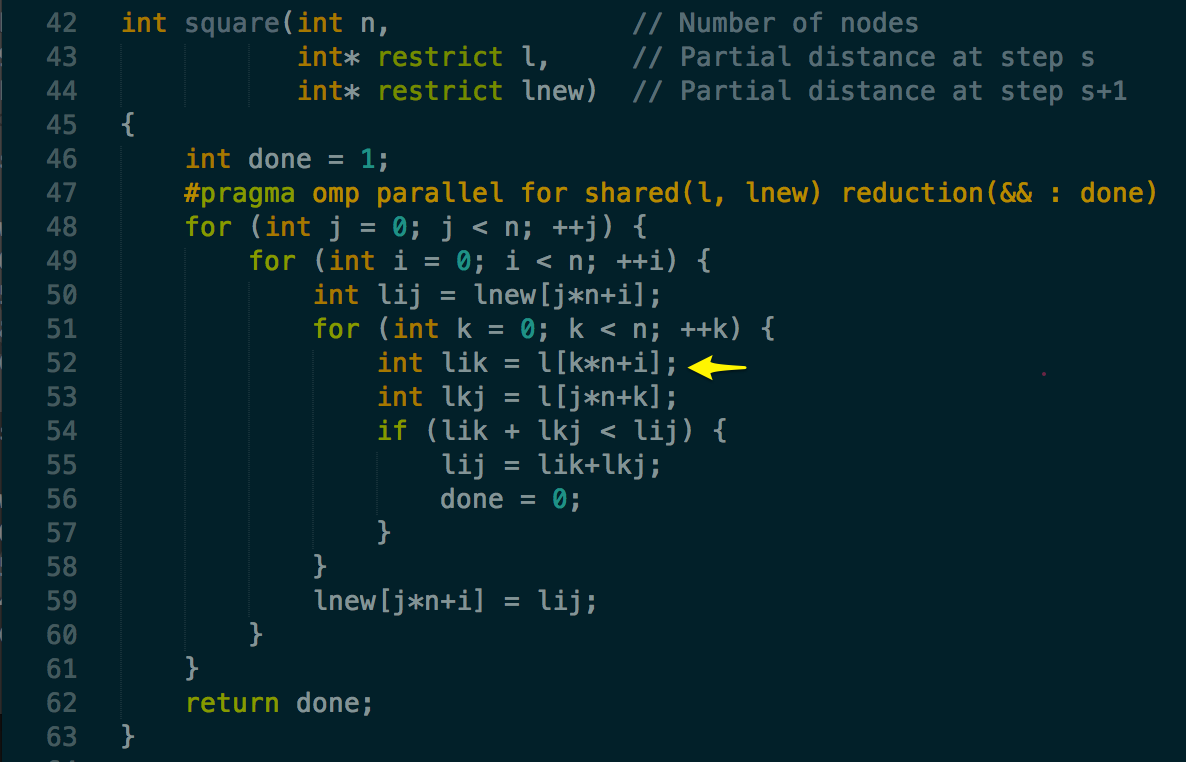
\includegraphics[width=0.7\tw]{fig-profile-bottlenecks-2.png}
  \caption{\textbf{function square, showing line numbers --}}
  \label{fig-profile-bottlenecks-2}
\end{figure}

From the original implementation of the code, we expected that the memcpy
from lnew to l after each iteration could potentially be rather expensive
-- especially as n becomes large. Since the results of each iteration
only depends on the matrix from the previous iteration (and not the
values from the current iteration), and given that we already have two
separate matrices, we could avoid this copying operation by swapping the
matrices between iterations -- reading from l and writing to lnew in one
iteration, and reading from lnew and writing to l in the next. In
practice however, this did not give us much speedup, due to the fact that
the actual number of iterations that the algorithm takes to converge is
rather low (for p = 0.05, and n = 2000, it typically converges within 2-4
iterations). This is also confirmed by the outputs from VTune profiling
reports, where for n = 10000, the CPU time used by memcpy (0.270s) is
rather insignificant as compared to the time spent in the functions
square (1368.604s, after tuning with copy optimization).

%\subsection{Performance Modeling}
%\label{sec-profile-modeling}
